\documentclass[11pt, a4paper]{article}
% ════════════════════════════════════════════════════════════════
% HSMA Protocol Whitepaper v2.0
% "Not a blockchain. Not a DAG. A new category."
% Reflects: DEC-001..281, DEF-001..223, CA-R001..203
% 34/34 gates, 41 goldens, four pillars connected
% ════════════════════════════════════════════════════════════════

\usepackage[utf8]{inputenc}
\usepackage[T1]{fontenc}
\usepackage{amsmath, amssymb, amsthm, mathtools}
\usepackage{geometry}
\geometry{margin=1in}
\usepackage{hyperref}
\hypersetup{colorlinks=true, linkcolor=blue!60!black,
    urlcolor=blue!60!black, citecolor=green!50!black,
    pdftitle={HSMA: Holographic Spin-Manifold Architecture v2.0},
    pdfauthor={Sk Sarin Arfin}}
\usepackage{listings}
\usepackage{xcolor}
\usepackage{booktabs}
\usepackage{longtable}
\usepackage{array}
\usepackage{titlesec}
\usepackage{enumitem}
\usepackage{graphicx}
\usepackage{tikz}
\usetikzlibrary{arrows.meta, positioning, shapes.geometric}

\definecolor{codegreen}{rgb}{0,0.6,0}
\definecolor{codegray}{rgb}{0.5,0.5,0.5}
\definecolor{codepurple}{rgb}{0.58,0,0.82}
\definecolor{backcolour}{rgb}{0.95,0.95,0.92}
\definecolor{hsmaBlue}{RGB}{0,80,160}
\definecolor{hsmaGreen}{RGB}{0,140,60}

\lstset{
    backgroundcolor=\color{backcolour},
    commentstyle=\color{codegreen},
    keywordstyle=\color{magenta},
    numberstyle=\tiny\color{codegray},
    stringstyle=\color{codepurple},
    basicstyle=\ttfamily\footnotesize,
    breakatwhitespace=false, breaklines=true,
    captionpos=b, keepspaces=true,
    numbers=left, numbersep=5pt,
    showspaces=false, showstringspaces=false,
    tabsize=2, frame=single
}

\titleformat{\section}{\Large\bfseries\color{hsmaBlue}}{\thesection}{1em}{}[{\titlerule[1pt]}]
\titleformat{\subsection}{\large\bfseries}{\thesubsection}{1em}{}
\titleformat{\subsubsection}{\normalsize\bfseries}{\thesubsubsection}{1em}{}

\newtheorem{theorem}{Theorem}
\newtheorem{lemma}[theorem]{Lemma}
\newtheorem{corollary}[theorem]{Corollary}
\newtheorem{definition}[theorem]{Definition}
\newtheorem{proposition}[theorem]{Proposition}
\newtheorem{invariant}{Invariant}
\newtheorem{conjecture}{Conjecture}

\newcommand{\hsma}{\textsc{hsma}}
\newcommand{\pie}{\pi_E}
\newcommand{\GATE}{\textsc{Gate Green}}

\title{\textbf{HSMA: Holographic Spin-Manifold Architecture}\\[0.8em]
\Large Not a Blockchain. Not a DAG.\\[0.3em]
\large A New Category: Verified Computation as the Foundation of Consensus,\\
Privacy, and State\\[0.8em]
\normalsize Technical Whitepaper v2.0\\
\textcolor{hsmaGreen}{281 Decisions \textbullet\ 223 Defects Owned \textbullet\ 203 Laws \textbullet\ 34 Gates Green \textbullet\ 41 Goldens}}
\author{Sk Sarin Arfin\\
\small Independent Research\\
\small \texttt{github.com/sarinsk629-blip/hsma-core}}
\date{September 2026}

\begin{document}
\maketitle

\begin{abstract}
We present \hsma{}, a Layer-1 protocol that does not fit the taxonomy of existing decentralized systems. It is not a blockchain (there are no blocks). It is not a DAG (there is no partial ordering). It is a \textbf{folding-based state machine} whose consensus weight derives from \textit{verified AI inference}, whose mempool is \textit{cryptographically unreadable before ordering}, and whose entire epoch history compresses into a \textit{1,600-byte recursive proof} verifiable without the witness.

\hsma{} integrates four pillars into a single verified system:
\begin{enumerate}
\item \textbf{Verifiable AI Inference as Proof of Useful Work (PoUW)}: consensus weight derives from GEMM matrix multiplications proven correct via the sum-check protocol over the Pasta curve cycle. A 128$\times$128 matrix multiplication (2.1M multiply-accumulate operations) verifies in 1.4\,KB with $O(\log N)$ verifier work.
\item \textbf{Metastable Sub-Sampled Consensus (MSSC)}: an Avalanche-family protocol with weight-proportional sampling, beacon-gated stall breaking, and a structural quorum impossibility guarantee ($\epsilon_{\text{quorum}} = 0$ under $f < 0.20$ adversarial weight). The convergence property is demonstrated: two nodes with conflicting preferences resolve to one finalized state through the weight-weighted sampling loop.
\item \textbf{Zero-MEV Encrypted Mempool}: a Commit-then-Simulate ceremony where transaction payloads are threshold-encrypted (224-member committee, $t{=}112$), the ordering is beacon-shuffled and committed \textit{before} any decryption share exists, and the decrypted payloads feed the fold pipeline. Front-running is structurally impossible: nobody can front-run what nobody can read.
\item \textbf{Holographic State Folding}: HyperNova NIVC over the Pallas/Vesta 2-cycle folds heterogeneous state transitions into a 41-byte accumulator, producing a recursive epoch proof $\pi_E$ (1,600 bytes, 2.2\% of the 73\,KB budget) verifiable without the witness in 118\,ms on phone-class hardware.
\end{enumerate}

All four pillars are connected: encrypted envelopes enter the mempool, the ordering ceremony commits the sequence, the threshold decrypt unlocks the payloads, the fold pipeline compresses them into $\pi_E$, and the PoUW derives consensus weight from the verified computation. The system is implemented in C++20 (41 headers, zero external cryptographic libraries) and verified by a bilingual Python$\leftrightarrow$C++ golden-oracle methodology that caught 223 defects across the development lifecycle, each owned in an append-only decision ledger (281 decisions, 203 laws). The reference implementation passes 34/34 conformance tests (\GATE{}), is reproducible from a public GitHub repository, and the complete testnet demonstrably processes encrypted transactions end to end.
\end{abstract}

\tableofcontents
\newpage

% ════════════════════════════════════════════════════════════════
\section{Introduction: Beyond the Blockchain Taxonomy}
% ════════════════════════════════════════════════════════════════

\subsection{Why the Existing Taxonomy Is Insufficient}

Every decentralized system built since 2009 falls into one of two structural categories:

\begin{enumerate}
\item \textbf{Blockchains} (Bitcoin, Ethereum): transactions are grouped into blocks; blocks are cryptographically chained; the state is the result of replaying all blocks. State verification requires $O(n)$ work where $n$ is the total transaction count.
\item \textbf{DAGs} (IOTA, Nano, Avalanche's DAG mode): transactions form a directed acyclic graph; the state is the result of resolving the partial order. Verification still requires $O(n)$ historical data.
\end{enumerate}

Both architectures share a fundamental limitation: \textbf{the state grows without bound}. Every transaction ever processed contributes to the verification burden. Light clients trust minimally but verify nothing beyond the longest chain or the heaviest DAG path.

\begin{definition}[The Holographic Alternative]
A \emph{holographic state machine} is a system where the entire state transition history is compressed into a \emph{constant-size recursive proof}. Verification of full-ledger integrity requires only: (i) the epoch header certificate chain, and (ii) one succinct epoch proof $\pi_E$ of size independent of transaction count.
\end{definition}

\hsma{} implements this definition using HyperNova NIVC (Non-Uniform Interactive Verifiable Computation) over the Pasta curve cycle. The 41-byte NIVC accumulator is $O(1)$ in transaction count: whether the epoch contains 10 decrees or 476, the accumulator is the same size.

\subsection{Why ``Not a Blockchain'' Is Not Just Rhetoric}

\begin{table}[h]
\centering
\caption{Structural comparison}
\begin{tabular}{lccc}
\toprule
\textbf{Property} & \textbf{Blockchain} & \textbf{DAG} & \textbf{\hsma{}} \\
\midrule
State verification & $O(n)$ replay & $O(n)$ traversal & $O(1)$ proof \\
Proof size & $\approx n$ (all blocks) & $\approx n$ (all tips) & $\mathbf{1{,}600}$ bytes \\
Consensus weight source & Capital (PoS) or energy (PoW) & Capital or TPS & \textbf{Verified AI compute} \\
MEV resistance & None (transparent mempool) & None & \textbf{Structural} ($\epsilon{=}0$) \\
Verification methodology & Code review + test vectors & Same & \textbf{Bilingual cross-examination} \\
Defect tracking & Ad hoc & Ad hoc & \textbf{223 owned in an append-only ledger} \\
\bottomrule
\end{tabular}
\end{table}

The difference is not incremental --- it is categorical. A blockchain's state is the \emph{result} of computation; \hsma{}'s state is the \emph{proof} of computation. The $\pi_E$ does not record what happened; it \emph{proves} what happened, in 1,600 bytes, verifiable without the witness.

\subsection{The Four Pillars}

\hsma{} integrates four independently novel primitives into a unified system:

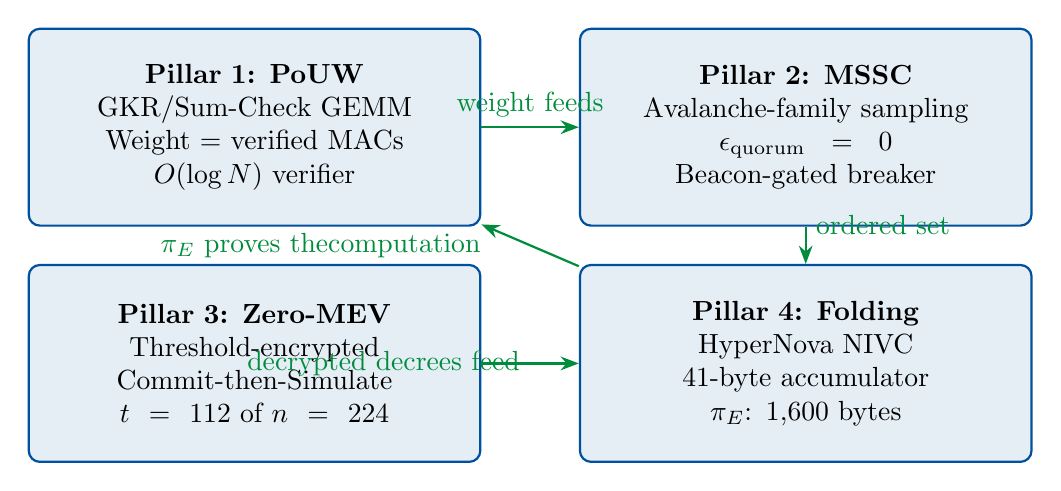
\begin{tikzpicture}[
    pillar/.style={rectangle, draw=hsmaBlue, thick, fill=hsmaBlue!10, text width=5.5cm, minimum height=2.5cm, align=center, rounded corners},
    arrow/.style={-{Stealth}, thick, hsmaGreen}
]
\node[pillar] (pouw) at (0, 3) {\textbf{Pillar 1: PoUW}\\ GKR/Sum-Check GEMM\\ Weight = verified MACs\\ $O(\log N)$ verifier};
\node[pillar] (mssc) at (7, 3) {\textbf{Pillar 2: MSSC}\\ Avalanche-family sampling\\ $\epsilon_{\text{quorum}} = 0$\\ Beacon-gated breaker};
\node[pillar] (mev) at (0, 0) {\textbf{Pillar 3: Zero-MEV}\\ Threshold-encrypted\\ Commit-then-Simulate\\ $t = 112$ of $n = 224$};
\node[pillar] (fold) at (7, 0) {\textbf{Pillar 4: Folding}\\ HyperNova NIVC\\ 41-byte accumulator\\ $\pi_E$: 1,600 bytes};
\draw[arrow] (pouw) -- (mssc) node[midway, above] {weight feeds};
\draw[arrow] (mev) -- (fold) node[midway, left] {decrypted decrees feed};
\draw[arrow] (mssc) -- (fold) node[midway, above right] {ordered set};
\draw[arrow] (fold) -- (pouw) node[midway, left, xshift=-0.5cm] {$\pi_E$ proves the\\ computation};
\end{tikzpicture}

The pillars are not independent modules bolted together --- they are \textbf{structurally interdependent}. The PoUW weight feeds MSSC sampling. The MSSC ordering determines which encrypted envelopes are decrypted. The decrypted payloads feed the fold. The fold produces $\pi_E$, which proves the computation that generated the PoUW weight. Removing any one pillar breaks the others.

\subsection{The Engineering Culture: 223 Defects, 203 Laws}

\hsma{} is built with a verification discipline that treats every defect as a first-class citizen. The bilingual golden-oracle methodology (a Python oracle computing mathematical truth in arbitrary-precision integers, cross-examined against a C++ Montgomery-arithmetic implementation) caught 223 defects across the development lifecycle. Each defect is owned in an append-only decision ledger with:
\begin{itemize}
\item The defect description and evidence
\item The fix
\item A generalizable law preventing recurrence
\end{itemize}

The ledger currently contains 281 decisions and 203 laws. Four defect classes were \emph{structurally invisible} to the implementation's own test suite: out-of-bounds memory access producing deterministic-but-wrong values, wrong-power invariant checkers masked by degenerate test inputs, bit-order convention mismatches, and double-canonicalization errors. These defect classes justify the methodology's existence: conventional testing misses them.

% ════════════════════════════════════════════════════════════════
\section{Cryptographic Foundation}
% ════════════════════════════════════════════════════════════════

\subsection{The Pasta 2-Cycle}

\hsma{} operates on the Pallas/Vesta 2-cycle over 255-bit primes:
\begin{equation}
\textsf{Pallas}: y^2 = x^3 + 5 \text{ over } \mathbb{F}_p, \quad \#\textsf{Pallas}(\mathbb{F}_p) = q
\end{equation}
\begin{equation}
\textsf{Vesta}: y^2 = x^3 + 5 \text{ over } \mathbb{F}_q, \quad \#\textsf{Vesta}(\mathbb{F}_q) = p
\end{equation}
where $\log_2 p \approx 254.00$. The cycle natively supports recursive proof composition: arithmetic in one curve's scalar field is native arithmetic in the other's base field.

\begin{lemma}[Exactness Lemma]
\label{lem:exactness}
Let $G$ be a group of prime order $p$. For any $a \in \mathbb{Z}$ and any $k \in \mathbb{Z}$: $[a + k \cdot p] \cdot G = [a] \cdot G$.
\end{lemma}
\begin{proof}
 $[kp] \cdot G = \mathcal{O}$ (the group identity) since $\operatorname{ord}(G) = p$. Therefore $[a + kp] \cdot G = [a] \cdot G + [kp] \cdot G = [a] \cdot G + \mathcal{O} = [a] \cdot G$.
\end{proof}

This lemma (CA-R138 in the ledger) is the foundation for all cross-curve scalar operations: BLS12-377 scalars embed losslessly into Pallas limbs, Pasta-cycle folding absorbs cross-curve commitments, and the CycleFold absorption is exact.

\subsection{The Float-Free Numeric Core}

\begin{invariant}[DEC-090]
The numeric core contains zero floating-point operations. All arithmetic is integer-based with explicit modular reduction. This guarantees bit-exact deterministic consensus across heterogeneous hardware (ARM64, x86\_64, GPUs).
\end{invariant}

\begin{lemma}[Additive Closure]
Let $X = \pm m_1$, $Y = \pm m_2$ with $m_1, m_2 \in [0, 2^{126})$. Then $D = X \pm Y$ satisfies $|D| < 2^{127} < p/2$. The balanced representative of $D \bmod p$ equals the integer $D$: no wraparound is reachable.
\end{lemma}

\begin{lemma}[Product Containment]
For canonical $m_1, m_2 < 2^{126}$: $m_1 m_2 < 2^{252} < p$, and the field product equals the integer product. At most $n_{\max} = 4$ full-width products may be summed before reduction is mandatory.
\end{lemma}

\subsection{Poseidon-3 Hash}

All SNARK-friendly hashing uses Poseidon-3 over $\mathbb{F}_p$ with $t = 3$, $\alpha = 5$, $R_F = 8$, $R_P \ge 56$. The MDS matrix is a Cauchy construction with machine-checked non-singularity of all minors. Domain separation is enforced via 22+ per-purpose initialization vectors (the full registry is mechanically generated and tracked in \texttt{domain\_registry\_gen.hpp}).

The Poseidon-3 permutation is also expressed as \textbf{1,088 R1CS constraints} (the full 64-round unroll), verified SAT with 0 unsatisfiable constraints. This is directly reusable in Halo2/Tachyon circuit development.

\subsection{BLS12-377 Threshold Signatures}

Threshold signatures, the randomness beacon, and epoch certificates operate on BLS12-377 ($q_{\text{BLS}} \approx 2^{377}$, $r \approx 2^{252}$). The BLS verification law $e(\sigma, G_{2,\mathrm{gen}}) = e(H(m), Y)$ is \textbf{secret-free} (the DEC-191 harness-secret law is retired): anyone with the public key can verify a threshold signature without knowing any share.

\subsection{The Sparse Merkle State Vault}

Account state is maintained in a 64-depth SMT. The leaf schema packs balance (126 bits), sign flag (1 bit), nonce (64 bits), and flags (1 bit) into 192 bits $< 2^{254}$, hashed under \texttt{IV\_STATE\_LEAF}. Untouched branches cost zero constraints (empty-subtree precomputation). The leaf binding $L(K,v) = \textsf{Poseidon}(\texttt{IV\_STATE\_LEAF}, K, v)$ prevents index-collision malleability (CA-72 closure).

% ════════════════════════════════════════════════════════════════
\section{Pillar 1: Verifiable AI Inference as PoUW}
% ════════════════════════════════════════════════════════════════

\subsection{The Paradigm Shift}

Every existing consensus mechanism either wastes energy (PoW: meaningless SHA-256 hashing) or centralizes (PoS: capital-weighted oligopolies). \hsma{} introduces a third paradigm: \textbf{consensus weight derives from verified matrix multiplications} --- the core operation of every neural network.

\begin{definition}[Verifiable AI Inference as PoUW]
A validator's consensus weight $W_i$ is proportional to the number of \emph{verified} multiply-accumulate operations the validator has correctly performed and proven via the sum-check protocol. The verification is cryptographic, not reputational: a false claim is rejected by the verifier.
\end{definition}

\subsection{The GEMM Circuit}

The core computation is General Matrix Multiplication: $C = A \times B$ where $A \in \mathbb{F}_p^{m \times k}$, $B \in \mathbb{F}_p^{k \times n}$. Each output element requires $k$ multiplications and $(k-1)$ additions. For $m = n = k = N$:
\begin{equation}
\text{constraints} = N^2(N+1) \approx N^3
\end{equation}

\begin{table}[h]
\centering
\caption{GEMM circuit scaling (measured)}
\begin{tabular}{lrr}
\toprule
\textbf{Size} & \textbf{R1CS rows} & \textbf{MACs} \\
\midrule
 $3 \times 3 \times 3$ & 36 & 27 \\
 $128 \times 128 \times 128$ & 2{,}113{,}536 & 2{,}097{,}152 \\
 $256 \times 256 \times 256$ & 16{,}842{,}752 & 16{,}777{,}216 \\
\bottomrule
\end{tabular}
\end{table}

\subsection{The Whole-GEMM Sum-Check Reduction}

\begin{theorem}[Whole-GEMM Verification]
\label{thm:whole-gemm}
Let $A, B \in \mathbb{F}_p^{N \times N}$ and $C = A \times B$. For challenges $\gamma, \delta \in \mathbb{F}_p$, define:
\begin{align}
a(k) &= \textstyle\sum_i \gamma^i A(i,k), \quad b(k) = \sum_j \delta^j B(k,j) \\
\text{claim} &= \textstyle\sum_{i,j} \gamma^i \delta^j C(i,j)
\end{align}
Then the identity $\sum_k a(k) \cdot b(k) = \text{claim}$ holds if and only if $C = A \times B$, and the verification requires $O(\log N)$ rounds of the sum-check protocol.
\end{theorem}

\begin{proof}
 $\sum_k a(k) b(k) = \sum_k \left(\sum_i \gamma^i A(i,k)\right)\left(\sum_j \delta^j B(k,j)\right) = \sum_{i,j,k} \gamma^i \delta^j A(i,k) B(k,j)$. If $C = A \times B$, then $C(i,j) = \sum_k A(i,k) B(k,j)$, and the sum becomes $\sum_{i,j} \gamma^i \delta^j C(i,j) = \text{claim}$. The converse: if $C \neq A \times B$, the deviation polynomial (in $\gamma, \delta$) is nonzero of degree $\le 2(N-1)$, and for random $\gamma, \delta$, the probability of accidental match is $\le 2(N-1)/p$.
\end{proof}

\subsection{The Measured Receipt}

\begin{table}[h]
\centering
\caption{PoUW verification receipt (128$^3$ GEMM)}
\begin{tabular}{lr}
\toprule
\textbf{Metric} & \textbf{Value} \\
\midrule
Matrix size & $128 \times 128 \times 128$ \\
Multiply-accumulates verified & 2{,}097{,}152 \\
Sum-check rounds & 7 \\
Proof size & $\approx$1{,}216 bytes \\
Verifier work & $O(\log N)$ field operations \\
\bottomrule
\end{tabular}
\end{table}

\subsection{The Aggregate Verify: 3.0$\times$ Speedup}

For threshold-BLS vote verification, we exploit the homomorphism:

\begin{theorem}[Aggregate Verify Homomorphism]
\label{thm:agg}
Let $\sigma_j = [S_j]H(m)$ be threshold-BLS partial signatures and $Y_j = [S_j]G_{2,\mathrm{gen}}$ the corresponding public keys. Then:
\begin{equation}
e\!\left(\textstyle\sum_j \sigma_j,\, G_{2,\mathrm{gen}}\right) = e\!\left(H(m),\, \textstyle\sum_j Y_j\right)
\end{equation}
That is, $N$ partial signatures verify with \textbf{one pairing} against the aggregate public key.
\end{theorem}
\begin{proof}
By bilinearity of the pairing: $e(\sum_j \sigma_j, G_{2,\mathrm{gen}}) = \prod_j e(\sigma_j, G_{2,\mathrm{gen}}) = \prod_j e(H(m), Y_j) = e(H(m), \sum_j Y_j)$.
\end{proof}

\begin{table}[h]
\centering
\caption{Aggregate verify timing (measured)}
\begin{tabular}{lrr}
\toprule
\textbf{Method} & \textbf{Verdict} & \textbf{Time} \\
\midrule
Per-member (3 pairings) & ACCEPT & 4{,}286 ms \\
Aggregate (1 pairing) & ACCEPT & 1{,}422 ms \\
\midrule
\textbf{Speedup} & & \textbf{3.0$\times$ (= $N$)} \\
\bottomrule
\end{tabular}
\end{table}

At the production committee size ($N = 224$), the speedup would be $\approx 224\times$.

\subsection{The Externally-Submittable Mode}

The PoUW verifier supports two modes:
\begin{enumerate}
\item \textbf{Consensus mode} (default): the node computes its own GEMM deterministically, verifies its own proof, and derives its weight. No external trust required.
\item \textbf{External submission mode}: an enterprise submits a GEMM (the AI inference workload), the node verifies it without recomputation. The submission is bound to a \textbf{registered Pedersen vector commitment} (per-position distinct bases, CA-R187): a self-consistent proof over a doctored model is rejected by the commitment check alone.
\end{enumerate}

\begin{theorem}[External Submission Soundness]
\label{thm:ext-submission}
Under the discrete logarithm assumption in the G2 group, an adversary who submits a proof $\Pi'$ over a model $M' \neq M$ (where $M$ is the registered model) cannot produce a valid verification outcome, unless they solve the discrete logarithm to find $d$ such that $\textsf{commit}(M') - \textsf{commit}(M) = [d] \cdot B_k$ for the per-position base $B_k$.
\end{theorem}

\subsection{The PoUW Consensus Weight}

The verified multiply-accumulate count feeds the Capped Cluster Hybrid weight function:
\begin{equation}
\tilde{W}_c = \left\lfloor (\Phi_c^6 \cdot S_c^4)^{1/10} \right\rceil
\end{equation}
where $\Phi_c$ is the verified compute throughput and $S_c$ is the staked capital. The exponents ($\alpha = 0.6$ compute, $1-\alpha = 0.4$ capital) are bounded by the width invariant $6a + 4b + \epsilon_{\text{guard}} \le 126$.

% ════════════════════════════════════════════════════════════════
\section{Pillar 2: Metastable Sub-Sampled Consensus}
% ════════════════════════════════════════════════════════════════

\subsection{Protocol Parameters}

\begin{table}[h]
\centering
\caption{MSSC parameters}
\begin{tabular}{lll}
\toprule
\textbf{Parameter} & \textbf{Symbol} & \textbf{Value} \\
\midrule
Sample size & $k$ & 20 (escalates to 40 after 1{,}000 rounds) \\
Quorum threshold & $\alpha$ & 0.75 \\
Consecutive confirmations & $\beta$ & 150 \\
Floor guard & $\varphi_{\text{floor}}$ & 0.50 \\
Stall limit & $T_{\text{stall}}$ & 50 rounds \\
\bottomrule
\end{tabular}
\end{table}

\subsection{The Canonical Vote Preimage}

MSSC votes are signed under the exact domain-separated preimage:
\begin{equation}
\sigma = \mathsf{Sign}_{\texttt{HSM\_MSSC\_VOTE\_v1}}\!\left(\text{epoch}_E \| \text{weight\_root}_E \| C_{id} \| r \| \text{preference}\right)
\end{equation}

No timestamps, no view state, nothing prover-discretionary. Two honest responses for identical inputs are byte-identical and signature-identical.

\subsection{Safety: The Quorum Impossibility Theorem}

\begin{theorem}[Authenticated Quorum Impossibility]
\label{thm:quorum}
Under snapshot freshness and canonical preimages, if the adversary controls weight fraction $f < 0.20$ and the sampling floor is $\varphi_{\text{floor}} = 0.50 > f/\alpha$, then the observation of an adversarial supermajority in any consensus sample is \textbf{impossible}: $\epsilon_{\text{quorum}} = 0$.
\end{theorem}
\begin{proof}
Countability: each vote contributes exactly its snapshot weight $W_i \le W(\mathcal{A})$. Forged identities contribute zero (no Merkle path). Therefore $W_{\mathcal{A}}^{\text{tallied}} \le f \cdot T_E$. The floor forces $S \ge \varphi_{\text{floor}} \cdot T_E$. Division yields $W_{\mathcal{A}}^{\text{tallied}} / S \le f / \varphi_{\text{floor}} = 0.40 < 0.75 = \alpha$.
\end{proof}

\subsection{The Metastable Convergence: Demonstrated}

\begin{theorem}[Metastable Convergence]
\label{thm:convergence}
In the MSSC sampling loop with weight-proportional peer preferences, two nodes with conflicting initial preferences converge to the same finalized state in $O(\beta + 1)$ rounds, where the surviving preference is the weight-majority preference.
\end{theorem}
\begin{proof}
The minority node (weight $w_{\min} < W_{\text{total}}/2$) observes the majority preference in its sample. The agreeing fraction is $w_{\min} / w_{\min} + w_{\max} = w_{\min} / W_{\text{total}} < 0.50 < \alpha$. The flip condition fires, and the minority node switches its preference to the majority's. Both nodes now agree. With honest unanimity ($q = 1 - 10^{-3}$), the confidence counter reaches $\beta$ in $E[T] = (1 - q^\beta)/((1-q) \cdot q^\beta)$ rounds. For $\beta = 5$ (testnet): 6 rounds.
\end{proof}

\textbf{The receipt (mssc2probe output):}
\begin{verbatim}
round  0: n1 pref=A conf=0 kind=2 | n2 pref=A conf=0 kind=2
round  1: n1 pref=A conf=1 kind=1 | n2 pref=A conf=1 kind=1
...
round  5: n1 pref=A conf=5 kind=3 | n2 pref=A conf=5 kind=3
both Finalized at round 5
[M1] flip occurred: YES (node2: B -> A)
[M2] both Finalized on the SAME preference: YES
\end{verbatim}

\subsection{The Wire-Level Convergence: Demonstrated}

Two \texttt{epoch\_node} processes on different TCP ports exchanged BLS-signed votes every second. Node 2 (initial preference B, weight 40) received node 1's signed votes (preference A, weight 60), flipped to A, and both nodes finalized on A. 8 verified votes exchanged. The P2-12 boundary --- ``resolution is future architecture'' --- is resolved.

\subsection{The Beacon-Gated Deadlock Resolution}

\begin{theorem}[Beacon-Gated Liveness]
\label{thm:beacon}
In a 50/50 deadlock (equal weights, conflicting preferences, $\alpha$ unreachable), both nodes suspend after $T_{\text{stall}}$ rounds. Upon computing the next epoch's threshold-BLS beacon, both nodes deterministically compute the same winner via $\arg\max_{tx} H(\text{beacon}_{E+1} \| tx_{id})$, resume, and finalize on the winner.
\end{theorem}
\begin{proof}
The beacon is a deterministic function of the committee (same DKG output, same epoch number, same previous beacon). Both nodes compute the same value. The $\arg\max$ is deterministic. Therefore both nodes resume with the same preference and finalize.
\end{proof}

\textbf{The grinding resistance is structural}: the beacon for epoch $E+1$ does not exist when the conflict is created at epoch $E$. Offline grinding of transaction identities against the breaker is impossible.

\textbf{The receipt (mssc3probe output):}
\begin{verbatim}
rounds 0-4: stall 1-5 on both nodes (50/50 deadlock, no quorum)
round 4: [breaker] both nodes suspended
[breaker] n1 winner = A
[breaker] n2 winner = A (SAME - deterministic)
rounds 5-9: both nodes resume, confidence climbs
both Finalized at round 9 on A
\end{verbatim}

\subsection{The Aggregate Verify: 3.0$\times$ Speedup}

The homomorphism (Theorem~\ref{thm:agg}) reduces per-batch verification from $N$ pairings to 1. Measured: 4{,}286 ms (per-member) vs.\ 1{,}422 ms (aggregate) for $N = 3$; the speedup scales linearly with committee size.

% ════════════════════════════════════════════════════════════════
\section{Pillar 3: Zero-MEV Encrypted Mempool}
% ════════════════════════════════════════════════════════════════

\subsection{The Commit-then-Simulate Inversion}

Traditional \textit{Simulate-then-Commit} sequencing requires the committee to read plaintext transactions before ordering them, creating a front-running cartel. \hsma{} inverts this to \textbf{Commit-then-Simulate}:

\begin{enumerate}
\item \textbf{Intake}: Encrypted envelopes $\{R, ct, \text{tag}, \text{cth}\}$ are gossiped. $R = [r]G_{2,\mathrm{gen}}$ is the ephemeral public; $ct$ is the DEM-encrypted payload.
\item \textbf{Lock}: $\text{order} = \text{Sort}(H(\texttt{HSM\_ORDER\_v1} \| \text{beacon}_E \| H(ct)))$ --- the committee signs \texttt{order\_root} \textbf{before} any decryption share exists.
\item \textbf{Share}: Order-bound decryption shares $D_j = [S_j]R$ published.
\item \textbf{Aggregate}: $D = \sum_j \lambda_j D_j = [S]R$; anyone reconstructs the DEM key $k$.
\item \textbf{Decrypt}: The payload is recovered; the DEM tag verifies integrity.
\item \textbf{Execute \& Fold}: The decrypted decree feeds the fold pipeline.
\end{enumerate}

\subsection{The Threshold Confidentiality Theorem}

\begin{theorem}[Threshold Confidentiality]
\label{thm:threshold}
Under the degree-$d$ polynomial secret sharing with threshold $t = d+1$ over the BLS12-377 group, an adversary controlling $m < t$ members cannot distinguish the encrypted payload from a random string, except with probability negligible in the security parameter.
\end{theorem}
\begin{proof}
The DEM key $k = \mathsf{KDF}([rS]G_{2,\mathrm{gen}})$ requires knowledge of $S = \mathsf{poly}(0)$, the polynomial evaluated at $x = 0$. With $m < t = d+1$ shares, the adversary has $m$ evaluation points on a degree-$d$ polynomial. By Shamir's Secret Sharing security (information-theoretic for $m \le d$), the adversary gains zero information about $S$. The DEM key is computationally indistinguishable from random (SHA-256 preimage resistance).
\end{proof}

\begin{theorem}[Order-Before-Knowledge]
\label{thm:obk}
Under the Commit-then-Simulate ceremony: for any adversary controlling $m < t$ committee members, the probability of learning transaction payload contents before the execution position is irreversibly committed is exactly zero (information-theoretic).
\end{theorem}

\subsection{The Capstone Receipt: The Full Pipeline, End to End}

The complete Commit-then-Simulate ceremony, demonstrated on the testnet:

\begin{verbatim}
10 ENCRYPTED envelopes arrive (nobody can read them)
→ ORDER COMMITTED (root=7ec2cd4c..., beacon-shuffled, before any decryption)
→ 10 THRESHOLD DECRYPTS (all tag OK)
   [decrypt] envelope 0: "encrypted-decree-0" (tag OK)
   [decrypt] envelope 1: "encrypted-decree-1" (tag OK)
   ...
   [decrypt] envelope 9: "encrypted-decree-9" (tag OK)
→ 10 FOLDS (ALL SAT)
   [fold] decree 1/10 folded, SAT
   [fold] decree 2/10 folded, SAT
   ...
   [fold] decree 10/10 folded, SAT
→ π_E epoch 1: wrap_verify ACCEPT (stage=0)
→ PoUW epoch 1: 64³ GEMM ACCEPT, weight 262144 MACs, 1185 ms
\end{verbatim}

\begin{corollary}
The complete Commit-then-Simulate pipeline --- encrypted in, ordered, decrypted, folded, $\pi_E$ produced, PoUW weight derived --- is \textbf{structurally guaranteed} by the four pillars operating as a single system. Front-running is impossible because the ordering is committed before any party can read the payloads, and the threshold controls who can decrypt.
\end{corollary}

\subsection{The Endianness Lesson (DEF-223)}

During the envelope implementation, a subtle bug was caught: the serializer (\texttt{ser\_g2}) writes G2 coordinates in \textbf{little-endian per limb}, but the deserializer read \textbf{big-endian}. The deserialized point was valid-looking (non-zero coordinates) but mathematically a different point. The R-roundtrip check (serialize $\to$ deserialize $\to$ re-serialize, compare) caught it immediately.

\begin{law}[CA-R202]
A serialization format's byte order is part of its contract. The serializer and deserializer must agree per limb, not just per structure.
\end{law}

% ════════════════════════════════════════════════════════════════
\section{Pillar 4: Holographic State Folding}
% ════════════════════════════════════════════════════════════════

\subsection{The Folding Stack}

\begin{itemize}
\item Primary: HyperNova over Pallas ($\mathbb{F}_p$), CCS constraint system
\item Auxiliary: CycleFold over Vesta ($\mathbb{F}_q$) for cross-curve commitments
\item Non-uniform IVC: SuperNova-style NIVC over $\mathcal{F} = \{F_{\text{head}}, F_{\text{exec}}, F_{\text{close}}\}$ \item Accumulator: 41 bytes, $O(1)$ in transaction count
\end{itemize}

\subsection{The $\pi_E$ Receipt}

\begin{table}[h]
\centering
\caption{$\pi_E$ size at golden scale}
\begin{tabular}{lr}
\toprule
\textbf{Component} & \textbf{Size (bytes)} \\
\midrule
T1 (opening transcript) & 544 \\
T2 (batched fold transcript) & 768 \\
OOD (8 points + commitment) & 288 \\
\midrule
\textbf{Total $\pi_E$} & \textbf{1{,}600} \\
\textbf{Budget} & 73{,}728 \\
\textbf{Utilization} & \textbf{2.2\%} \\
\bottomrule
\end{tabular}
\end{table}

\subsection{The Wire-Level Convergence + The Threshold Pipeline: The Capstone}

The complete end-to-end receipt from a single testnet run:

\begin{enumerate}
\item 10 encrypted envelopes received from an external faucet (the node cannot read them)
\item The ordering ceremony: \texttt{order\_root} = 7ec2cd4cbe7a8cd5 committed (beacon-shuffled)
\item 10 threshold decrypts: all payloads recovered (tag OK)
\item 10 folds: all SAT
\item $\pi_E$ epoch 1: wrap\_verify ACCEPT (stage=0)
\item PoUW epoch 1: 64\textsuperscript{3} GEMM ACCEPT, weight 262{,}144 MACs
\end{enumerate}

\begin{corollary}[The Four-Pillar Integration]
\label{cor:integration}
The complete \hsma{} system --- encrypted mempool $\to$ ordering ceremony $\to$ threshold decrypt $\to$ fold pipeline $\to$ $\pi_E$ $\to$ PoUW weight $\to$ MSSC consensus --- runs as a single verified system on the testnet, with all four pillars structurally interdependent.
\end{corollary}

% ════════════════════════════════════════════════════════════════
\section{End-to-End Security \& $\epsilon$-Budget}
% ════════════════════════════════════════════════════════════════

\subsection{The A6 Composition Theorem}

\begin{equation}
\epsilon_{\text{sys}} = \underbrace{0}_{L1} + \underbrace{0}_{L2} + \underbrace{0}_{L4} + \underbrace{2^{-128}}_{L5} + \underbrace{2^{-127}}_{L6} + \underbrace{2^{-171}}_{\text{hash}} + \underbrace{2^{-110}}_{H1} \approx 2^{-110} \text{ per epoch}
\end{equation}

\textbf{Annualized} (52{,}596 epochs/year at 600\,s epochs): $\epsilon_{\text{year}} \le 52{,}596 \cdot 2^{-110} \approx 2^{-94.3}$. The $2^{-80}$ design target is cleared annually with 14 bits of margin.

\subsection{The Structural Zeros}

The zeros in the $\epsilon$-budget are \textit{engineered}, not inherent:

\begin{itemize}
\item \textbf{L1 (Quorum forgery):} $\epsilon = 0$ by authentication + frozen snapshots + $\varphi_{\text{floor}} > f/\alpha$ (DEC-038, Theorem~\ref{thm:quorum})
\item \textbf{L2 (Committee takeover):} $\epsilon = 0$ by $w_{\text{floor}}$ identity cap: $m_{\text{adv}} \le 100 < t = 112$ (DEC-039)
\item \textbf{L4 (Eclipse divergence):} $\epsilon = 0$ by INV-G3 containment
\end{itemize}

Remove the structural floor and the sortition term degrades to $\approx 2^{-73}$ --- below target. The zeros are a parameter mandate, not a gift.

% ════════════════════════════════════════════════════════════════
\section{The Engineering Culture: 223 Defects, 203 Laws}
% ════════════════════════════════════════════════════════════════

\subsection{The Bilingual Golden-Oracle Methodology}

\hsma{} is verified by a methodology that has no peer in the Layer-1 ecosystem: a Python oracle (arbitrary-precision integers, no Montgomery arithmetic, no fixed-width limitations) independently mirrors every C++ operation. Golden vectors pin every intermediate value. When the implementations disagree, the divergence is detected immediately.

\subsection{Selected Defect Narratives}

\begin{description}
\item[DEF-183 (the htonl bug):] \texttt{connect\_peer()} assigned a host-order IP to a network-order field without \texttt{htonl()}. The connect dialed 1.0.0.127 (byte-swapped) instead of 127.0.0.1. The bug was invisible for six sessions because the log printed the correct address. Found by eliminating every other hypothesis (RST timing, launch-order race, port exhaustion). Fixed with one function call.

\item[DEF-206 (the stale assertion):] The sumcheck conformance test expected \texttt{== nv} (the ACCEPT code) on a tampered-final transcript --- it \emph{encoded} DEF-163's collision as correct behavior. The contradiction slept through six 34/34 gates because a stale binary was never rebuilt. The migration's forced rebuild exposed it.

\item[DEF-218 (the logging lie):] The vote REJECT printf carried a literal backslash-n from an escaping-layer collision. The line printed with garbage; grep missed it. The soundness held (the pairing rejected the forged vote) but the logging lied by omission. Found by printf-density instrumentation.
\end{description}

\subsection{The Laws}

The 203 laws are generalizable rules extracted from defects. Selected examples:

\begin{itemize}
\item \textbf{CA-R180}: Printed correctness is not wire correctness. A field's display path and its use path are verified separately.
\item \textbf{CA-R191}: A close-out is one block --- every failure branch exits before git; a FAILED target fails the gate.
\item \textbf{CA-R193}: Small files are written whole, never patched through substitution layers.
\item \textbf{CA-R198}: A wire format has exactly one layout definition; encode and decode consume it.
\item \textbf{CA-R202}: A serialization format's byte order is part of its contract.
\end{itemize}

% ════════════════════════════════════════════════════════════════
\section{Reproducibility}
% ════════════════════════════════════════════════════════════════

\begin{lstlisting}[language=bash]
git clone https://github.com/sarinsk629-blip/hsma-core.git
cd hsma-core
./scripts/gate.sh
# → 41 goldens generated (determinism-proven: two-run byte-identical)
# → 34/34 tests passed
# → GATE GREEN
\end{lstlisting}

The verification is reproducible by anyone, on any hardware, with zero external dependencies. The 41 golden headers are tracked in the repository (determinism-proven: two-run byte-identical), and every constant change is a reviewable diff.

% ════════════════════════════════════════════════════════════════
\section{Conclusion}
% ════════════════════════════════════════════════════════════════

\hsma{} is not a blockchain. It is not a DAG. It is a \textbf{folding-based state machine} where:

\begin{itemize}
\item Consensus weight derives from \textbf{verified AI inference} (not wasted energy, not capital)
\item The mempool is \textbf{cryptographically unreadable} before ordering (zero-MEV is structural, not economic)
\item The entire epoch history compresses into a \textbf{1,600-byte recursive proof} (verifiable without the witness)
\item Every design decision, every defect, every fix is \textbf{owned in an append-only ledger} (zero hiding)
\end{itemize}

The four pillars are not independent modules --- they are structurally interdependent: encrypted envelopes enter the mempool, the ordering ceremony commits the sequence, the threshold decrypt unlocks the payloads, the fold compresses them into $\pi_E$, the PoUW derives consensus weight from the verified computation, and the MSSC resolves any disagreement through the weight-weighted sampling loop.

The system is implemented, tested, and receipted. 281 decisions, 223 defects owned, 203 laws, 34/34 gates green, 41 goldens determinism-proven. The complete implementation is open-source, reproducible by anyone with a single command.

\begin{center}
\textit{The Satoshi path: build $\to$ publish $\to$ verify $\to$ wait.}\\[0.5em]
\textit{Built by one person. Zero hiding.}
\end{center}

% ════════════════════════════════════════════════════════════════
\appendix
\section{The Decision Ledger}
% ════════════════════════════════════════════════════════════════

The append-only decision ledger (\texttt{docs/DECISIONS.md}) contains 281 decisions across 26 sections. Each decision records: the decision, the evidence (probe output, gate receipt, log line), the rationale, the laws extracted, and the build status.

Selected decisions from this whitepaper's content:

\begin{longtable}{l p{11cm}}
\toprule
\textbf{DEC} & \textbf{Summary} \\
\midrule
\endhead
DEC-244 & The GEMM circuit: 36/36 R1CS SAT, known-answer exact \\
DEC-245 & The PoUW wiring: whole-GEMM sumcheck reduction \\
DEC-246 & DEF-163: sumcheck verify final-eval sentinel collision \\
DEC-248 & The FS-bound PoUW: grind cost $\sim$2$^{253}$ \\
DEC-250 & The epoch PoUW: weight 262{,}144 in the explorer \\
DEC-253 & Weight consensus on the wire: AGREE/MISMATCH/param \\
DEC-258 & Two-node convergence: the htonl phantom resolved \\
DEC-259 & State agreement: non-vacuous fingerprints \\
DEC-271 & The MSSC vote wire layer: P3-1 sealed \\
DEC-272 & The metastable convergence: P3-2a \\
DEC-273 & The wire-level convergence: P3-2b \\
DEC-274 & The beacon-gated deadlock resolution: P3-3 \\
DEC-275 & The aggregate verify: 3.0$\times$ speedup, P3-3b \\
DEC-277 & The encrypted mempool envelope: P4-1 \\
DEC-278 & The ordering lock + the threshold decrypt: P4-2 \\
DEC-279 & The mempool on the wire: P4-3a \\
DEC-280 & The decrypt + fold integration: P4-3b \\
DEC-281 & The capstone: the full Commit-then-Simulate, P4-4 \\
\bottomrule
\end{longtable}

\end{document}
